\special{dvipdfmx:config z 0}
\documentclass[punct=CCT]{ctexbeamer}
\xeCJKEditPunctStyle{CCT}{bound-punct-ratio=0.5}
\usepackage{graphicx}

\usepackage{tabularray}
\usepackage{tcolorbox}
\usepackage{mathtools}
\usepackage{fixdif}
\usepackage{tensor}
\usepackage{cncolours}
\usepackage{physics2}
\usepackage{siunitx}
\usepackage{codehigh}
\usepackage{tikz-feynman}
\usephysicsmodule{braket}
\usepackage{twemojis}
\tcbuselibrary{skins}
\usepackage{%
    fontawesome5,
    hologo,
    bookmark,
    listings,
    multicol,
    qrcode,
    ragged2e,
    siunitx,
    xeCJKfntef,
    unicode-math,
    simpleicons
}

\usepackage{unicode-math}
\usepackage{tikz}
\UseTblrLibrary{booktabs}
\ctexset{today=big}
\usetheme[progressbar=frametitle, sectionpage = progressbar]{metropolis}



% \usetheme{Xiaoshan}
\usefonttheme{serif,professionalfonts}
\usetikzlibrary{decorations,decorations.markings}

\makeatletter

\apptocmd{\beamer@@frametitle}{%
  \only<1>{\expandafter\ifnum\insertcontinuationcount<2\relax
    \bookmark[page=\the\c@page,level=4]{#1}\fi}}{}{}
\DeclareRobustCommand{\LaTeX}{L\kern-.3em\raisebox{.2em}{\textsc{a}}\kern-.14em\TeX}
\DeclareRobustCommand{\LaTeXe}{%
\LaTeX\kern.15em2%
\hbox{%
\if b\expandafter\@car\f@series\@nil
$_{\textstyle\symbf{\varepsilon}}$%
\else
$_{\textstyle\varepsilon}$%
\fi}}

\newcommand \given{}
\newcommand \setskip{\mathchoice{\,}{\,}{\mkern1mu}{\mkern1mu}}
\newcommand \SetSymbol[1][]{%
\mkern1mu\nonscript\setskip#1\vert
\allowbreak
\nonscript\setskip\mkern1mu
\mathopen{}}
\DeclarePairedDelimiterX\@set[1]{\{}{\}}%
{\renewcommand\given{\SetSymbol[\delimsize]}%
\setskip#1\setskip\mathopen{}}
\DeclareDocumentCommand{\@set@nostar}{O{}O{\mathchoice{\,}{\,}{\mkern1mu}{\mkern1mu}}m}{%
\renewcommand{\setskip}{#2}\@set[#1]{#3}}
\DeclareDocumentCommand{\@set@star}{O{\mathchoice{\,}{\,}{\mkern1mu}{\mkern1mu}}m}{%
\renewcommand{\setskip}{#1}\@set∗{#2}}
\newcommand\set{\@ifstar\@set@star\@set@nostar}
\newcommand{\nonumberfootnote}[2][]{%
  \let\thefootnote\relax
  \footnotetext#1{\kern-.8\ccwd#2}}
\renewcommand{\footnoterule}{}
\newcommand\mathfontlist[1]{%
    \begin{matrix}
        \symup{#1}   & \symbf{#1}    & \symsf{#1}    & \symbfsf{#1}                          \\
        #1           & \symbfit{#1}  & \symsfit{#1}  & \symbfsfit{#1}                        \\
        \symcal{#1} & \symbfcal{#1} & \symbb{#1}    & \text{\mathversion{bold}$\symbb{#1}$} \\
        \symscr{#1} & \symbfscr{#1} & \symfrak{#1} & \symbffrak{#1}
    \end{matrix}%
}

\makeatletter
\renewenvironment{proof}[1][\proofname]{%
\par
  \def\insertproofname{#1\@addpunct{.}}%
  \pushQED{\qed}
  \alert{\insertproofname} \hspace*{\fill} \\ \kaishu}
{\popQED\par}
\makeatother

% \mode<presentation>
% \setbeamercolor{frametitle}{parent=palette primary}
% \setbeamercolor{subsection in head/foot}{parent=palette secondary}
% \setbeamercolor{section in head/foot}{parent=palette quaternary}

% \definecolor{def}{HTML}{000000}
% \definecolor{pri}{HTML}{0F4C75}
% \definecolor{sec}{HTML}{3282B8}
% \definecolor{ter}{HTML}{BBE1FA}
% \definecolor{ale}{HTML}{FF4E27}



% \setbeamercolor{title separator}{fg=靛蓝}
% \setbeamercolor{author}{fg=靛青}
% \setbeamercolor{institute}{fg=靛青}
% \setbeamercolor{date}{fg=靛青}

% \setbeamercolor*{palette primary}{fg=white,bg=pri}
% \setbeamercolor*{palette secondary}{fg=white,bg=靛蓝}
% \setbeamercolor*{palette tertiary}{fg=海棠红,bg=ter}

% \setbeamercolor{alerted text}{fg=ale}

% \mode<all>

\setCJKmainfont{Noto Serif CJK SC Medium}[
    BoldFont=Noto Serif CJK SC Bold,
    ItalicFont = 楷体,
    Script=CJK Ideographic, Language=Chinese Simplified
    ]
\setCJKsansfont{Sarasa Fixed Slab SC}
\setCJKmonofont[AutoFakeSlant]{Sarasa Fixed Slab SC}

\setmainfont{MinionPro-Subh}[BoldFont = MinionPro-BoldSubh, Letters = Uppercase]
\setsansfont{FiraGO Book}[Letters = Uppercase]
\setmonofont[Scale=.95,  Letters = Uppercase, BoldFont=Victor Mono Bold]{Victor Mono Medium}

\newfontfamily\tocsans{FiraGO ExtraLight}
\newCJKfontfamily\tocsansCJK{Sarasa Fixed Slab SC Light}
\newCJKfontfamily\NotoSerifCJKTC{Noto Serif CJK TC Medium}


    
\setmathfont[version = ltm]{NewCMMath-Regular.otf}
\setmathfont{MinionMath-Subh.otf}
[   
    SizeFeatures = {
        {Size = -6, Font = MinionMath-capt.otf,
        Style = MathScriptScript},
        {Size = 6-8.4, Font = MinionMath-regular.otf,
        Style = MathScript},
        {Size = 8.4-12, Font = MinionMath-Subh,
        Style = MathScript},
        {Size = 12-, Font = MinionMath-Disp.otf},
},
]
\setmathfont[version = bold]{MinionMath-Bold.otf}
[   
    SizeFeatures = {
        {Size = -6, Font = MinionMath-Bold.otf,
        Style = MathScriptScript},
        {Size = 6-8.4, Font = MinionMath-Bold.otf,
        Style = MathScript},
        {Size = 8.4-13, Font = MinionMath-Bold,
        Style = MathScript},
        {Size = 13-, Font = MinionMath-BoldSubh.otf},
    },
]
\setmathfont[range={sfup,sfit,bfsfup,bfsfit}]{Garamond-Math.otf}
\setmathfont[range={up/Greek,"2211, "220F}]{euler.otf}
\setmathfont[range={cal,frak,bfcal,bffrak}]{euler.otf}
\setmathfont[range={bfsfit/{greek, Greek},scr,bfscr}]{Garamond-Math.otf}
\setmathfont[range={"222B,"222C,"222D,"2A0C, },StylisticSet ={7,9}]{Garamond-Math.otf}
\setmathfont[range={}]{MinionMath-Subh.otf}

\DeclareGraphicsExtensions{.eps,.ps,.jpg,.bmp,.png}


\setbeamerfont{title}{size=\huge, series=\bfseries}
\setbeamerfont*{subtitle}{size=\large, shape=\itshape}
\setbeamerfont{section title}{size=\Large, series=\bfseries}
\setbeamerfont{frametitle}{size=\large, series=\bfseries}
\setbeamerfont{caption}{size=\footnotesize, series=\bfseries}
\setbeamerfont{itemize/enumerate subbody}{size=\footnotesize}
\setbeamerfont{footnote}{size=\tiny}
\setbeamerfont{author}{size=\small, shape=\scshape}
\setbeamerfont{institute}{size=\tiny}
\setbeamerfont{date}{size=\footnotesize}
\setbeamerfont{alerted text}{series=\bfseries}
\setbeamerfont{block title}{size=\small, series=\sffamily}

\setbeamertemplate{title}{%
    \linespread{1}%
    \inserttitle
    \hspace*{1.2cm}\par
    \vspace*{0.5em}}
\setbeamertemplate{date}{%
    \linespread{1}%
    \hspace*{0cm}\insertdate\par
    \vspace*{1.65em}}
\setbeamertemplate{author}{%
    \linespread{1}%
    \hspace*{0cm}\insertauthor\par}
\setbeamertemplate{institute}{%
    \linespread{1}%
    \hspace*{0cm}\insertinstitute\par
    \vspace*{0.5em}}
\setbeamertemplate{subtitle}{%
    \insertsubtitle
    \hspace*{1.2cm}\par
    \vspace*{0.5em}}
\setbeamertemplate{title page}{%
    \begin{minipage}[b]{\textwidth}
        \usebeamertemplate*{title}
        \usebeamertemplate*{subtitle}
        \usebeamertemplate*{title separator}
        \usebeamertemplate*{title graphic}
        \usebeamertemplate*{author}
        \usebeamertemplate*{date}
        \usebeamertemplate*{institute}
        \vfill
    \end{minipage}}
\setbeamertemplate{title graphic}{%
    \vbox to 0pt {\hfill\smash{\raisebox{-1cm}{\inserttitlegraphic}}}%
    \nointerlineskip}
\setbeamertemplate{frame numbering}{\zhnumber[style=Financial]{\insertframenumber}}
\setbeamertemplate{caption}{\parbox{\textwidth}{\centering\insertcaption}\par}
\setbeamertemplate{bibliography item}[text]
\setbeamerfont{bibliography item}{size=\fontsize{6}{8}}
\setbeamerfont{bibliography entry author}{size=\fontsize{6}{8}}
\setbeamerfont{bibliography entry title}{size=\fontsize{6}{8}}
\setbeamerfont{bibliography entry location}{size=\fontsize{6}{8}}
\setbeamerfont{bibliography entry note}{size=\fontsize{6}{8}}
\setbeamertemplate{blocks}[default]
\setbeamercolor{block title}{fg=white}

\AtBeginEnvironment{theorem}{\setbeamercolor{block title}{fg=white}}
\AtBeginEnvironment{axiom}{\setbeamercolor{block title}{fg=white}}
\AtBeginEnvironment{example}{\setbeamercolor{block title}{fg=white}}
\AtBeginEnvironment{block}{\setbeamercolor{block title}{fg=white}}

\setbeamertemplate{section in toc}{\vbox{\sffamily\tocsans\tocsansCJK\inserttocsection}\par\medskip}

\setbeamercolor{block body}{parent=normal text,use=block title,bg=block title.bg!10!bg}
\setbeamercolor*{block title}{bg=海棠红}
\setbeamercolor{normal text}{fg=黑色}
\setbeamercolor{alerted text}{fg=酡红}
\setbeamercolor{example text}{fg=靛蓝}

\title{实用主义家用 \LaTeX{} 入门}
\subtitle{\LaTeX{} \textit{for} Pragmatists}
\author{Innocent, Panadol}
\institute{中山大学\quad 笃行工作室 \textit{\&} SPS 物理协会}
\date{二〇二三年十二月八日}
\titlegraphic{%
\begin{minipage}{1.6cm}
    \centering\scriptsize
    \qrcode[hyperlink, height=1.6cm]{https://github.com/InnocentFIVE/LaTeX-Lecture-SPS-and-Duxing}\smallskip

    GitHub 链接
\end{minipage}\kern\ccwd
\begin{minipage}{1.6cm}
    \centering\scriptsize
    \qrcode[hyperlink, height=1.6cm]{https://qm.qq.com/q/6vdDIExV0Q}\smallskip

    QQ 交流群
\end{minipage}}

\colorlet{keyword}{松柏绿}
\colorlet{comment}{漆黑!50}
\colorlet{texcs}{妃色}
\colorlet{emph1}{靛青}
\colorlet{emph2}{琥珀}
\colorlet{emphbig}{酡颜}
\colorlet{emphBig}{酡颜!80!漆黑}
\colorlet{emphbigg}{酡颜!60!漆黑}
\colorlet{emphBigg}{酡颜!40!漆黑}
\colorlet{inline}{苍色!80!靛青!70!漆黑}

\usepackage{etoolbox}
\makeatletter
\patchcmd{\beamer@tableofcontents}{%
\vspace *{-.5em}}{}{}{}
\patchcmd{\beamer@sectionintoc}{\def \beamer@breakhere {\\}}{\def \beamer@breakhere {}}{}{}
\patchcmd{\beamer@sectionintoc}{\ifx \beamer@toc@ooss \beamer@hidetext \vskip 1.5em \else \vfill \fi}{}{}{}
\patchcmd{\beamer@sectionintoc}{\hbox}{}{}{}
\patchcmd{\beamer@sectionintoc}{\vbox}{}{}{}
\AddToHook{cmd/tableofcontents/before}{\mbox{}\vskip-\baselineskip}
\setlength{\metropolis@progressonsectionpage@linewidth}{4pt}
\setlength{\metropolis@progressinheadfoot@linewidth}{2pt}


\lstdefinestyle{style@latex}{
    language     = [latex]TeX,
    alsoletter   = {*},
    keywordstyle = \bfseries\color{keyword},
    commentstyle = \itshape\color{comment},
    texcsstyle   = *\color{texcs},
    emphstyle    = [1]\itshape\color{emph1},
    emphstyle    = [2]\color{emph2},
    emphstyle    = [11]\color{emphbig},
    emphstyle    = [12]\color{emphBig},
    emphstyle    = [13]\color{emphbigg},
    emphstyle    = [14]\color{emphBigg},
}
\lstdefinestyle{style@inline}{
  basicstyle   = \ttfamily\color{inline},
  keepspaces   = true,
}
\lstdefinestyle{style@pkg}{
  basicstyle   = \sffamily\color{inline},
  keepspaces   = true,
}
\lstnewenvironment{texcode}[1][]{\lstset{
  style        = style@latex,
  escapeinside = {\%*}{*)},
  morekeywords = {\documentclass,\usepackage,\begin,\end},
  basicstyle   = \footnotesize\ttfamily,
  basewidth    = .57\ccwd,
  literate     = 
    {&}{{\textcolor{蔚蓝!80!blue}{\&}}}1
    {$}{{\textcolor{粉红}{\$}}}1,
    #1}}{}
\lstMakeShortInline[style=style@inline]|

\newcommand{\pkg}[1]{\href{https://ctan.org/pkg/#1}{\textsf{\addfontfeatures{RawFeature=-case}#1}}}


\ExplSyntaxOn
\xeCJK_new_class:n { PoZheHao }
\__xeCJK_save_CJK_class:n { PoZheHao }
\xeCJK_declare_char_class:nn { PoZheHao } { "2014 }
\seq_map_inline:Nn \g__xeCJK_class_seq
  {
    \str_if_eq:nnF {#1} { PoZheHao }
      {
        \xeCJK_copy_inter_class_toks:nnnn { PoZheHao } {#1} { FullRight } {#1}
        \xeCJK_copy_inter_class_toks:nnnn {#1} { PoZheHao } {#1} { FullRight }
      }
  }
\ExplSyntaxOff

\newcommand{\link}[1]{\href{#1}{\faLink}}




\newtheorem{axiom}{公理}


\newcommand{\XeLaTeX}{\hologo{Xe}\kern-.13em\LaTeX{}}
\newcommand{\pdfLaTeX}{pdf\LaTeX{}}
\newcommand{\LuaLaTeX}{Lua\LaTeX{}}
\newcommand{\BibTeX}{B\kern-.05em\textsc{i\kern-.025em b}\kern-.08em\TeX{}}
\NewDocumentCommand{\sectionwithabstract}{o m o}{%
\begin{frame}[noframenumbering]
    \thispagestyle{empty}
	\centering
	\IfValueTF{#1}{\section[#1]{#2}}{\section{#2}}
    \vskip-.5\baselineskip
	\IfValueT{#3}{\begin{minipage}[t][0pt][t]{22em}\footnotesize
		#3
	\end{minipage}}
	\vskip-1.5\baselineskip
	\vskip-\parskip
	\vskip-6pt
\end{frame}%
}
\NewDocumentCommand{\DifficultyOfEditor}{m m m m}{%
	\Large\makebox[#1\ccwd][r]{\fontspec{RevueEF.otf}#2}\kern\ccwd #3\par
    \hspace*{#1\ccwd}\kern\ccwd\footnotesize #4\par%
}

\newcommand{\JPtext}[1]{{\addCJKfontfeatures{Language=Japanese}#1}}

\usepackage{fbox}
\newcommand*\ideographicbaseline{-0.12}
\newcommand*\ccbox[1][1]{%
    \smash{%
    \rlap{%
        \color{gray}%
        \setlength\fboxrule{0.4pt}%
            \setlength\fboxsep{-.5\fboxrule}%
            \fbox{%
                \rule[\ideographicbaseline\ccwd]{0pt}{\ccwd}%
                \rule{#1\ccwd}{0pt}%
            }% 
        }%
    }%
    \kern#1\ccwd
}
\begin{document}
\maketitle


\begin{frame}
	\begin{columns}[t]
		\begin{column}{.3\textwidth}
			\par\medskip
			\Huge\hfill\hbox{\smash{\parbox[b]{\ccwd}{\linespread{1}\selectfont 目录~\smash{\usebeamercolor[fg]{alerted text}\rule[-.12\ccwd]{.4pt}{2.12\ccwd}}}}}
		\end{column}
		\begin{column}{.65\textwidth}
			\tableofcontents
		\end{column}
	\end{columns}
\end{frame}

\sectionwithabstract{从零}[\NotoSerifCJKTC 萬物是藉著他造的;凡被造的,沒有一樣不是藉著他造的.\\\mbox{}\hfill ---\textsc{John 1:3}. \emph{The Word Became Flesh}%
]

\begin{frame}{实用主义者的自白}
	\pause 在一切一切开始之前……我们用最简洁的方式来介绍 \LaTeX{},我们将会:\pause
	\begin{itemize}
		\item<+-> 给出写出一篇(最基本的)文档的方法,将更具体的\LaTeX{}特性阐释后置;
		\item<+-> 也许你会说:“\alert{我还不知道\LaTeX{}怎么下载呢!}”别急,我们将会使用在线的 TeXPage;
		\item<+-> 在这个阶段,我说的话可能是有失偏颇的……但说得太多可能会引发初学者的畏难情绪,而这在一开始是没有必要的;
		\item<+-> 总而言之,先让它动起来再说.
	\end{itemize}
\end{frame}

\begin{frame}{简要的介绍}
    \begin{itemize}
        \item<+-> \LaTeX{} 是什么?
        \begin{itemize}
            \item<+-> 粗略来说,是 Leslie Lamport 对 \TeX{} 的一种封装;
            \item<+-> “排版公式很厉害且写论文 / 提交作业要用的”的排版系统;
            \item<+-> 从嘴里说出来时,\LaTeX{}(大概)是\TeX{}、\LaTeX{}内核、文档类、宏包的总称;
            \item<+-> \LaTeX{} 语法是数学家之间的交流方式.
        \end{itemize}
        \item<+-> \TeX{} 是什么?
        \begin{itemize}
            \item<+-> Donald~E.\ Knuth 和他的学生开发的排版文字和数学公式而开发的排版引擎;
            \item<+-> \LaTeX{} 的底层,真正负责排版的东西.
        \end{itemize}
    \end{itemize}
\end{frame}



\begin{frame}[t,fragile]{演示:\LaTeX{},启动!}
    按照惯例,我们先来给出我们的第一篇文档(还有最基本的中英混排的例子).\pause 
	\begin{texcode}[emph={[1]document}, emph={[2]article}]
    \documentclass{article}
    % 这里是导言区,% 用来表示注释
    \begin{document}
    Hello, world!
    \end{document}
\end{texcode}\pause 
    \begin{itemize}
        \item<+-> 其中,|\documentclass| 是一个控制序列,|{article}| 是其的一个必要参数,参数值是 |article|,表示调用 \pkg{article} 文档类.

        \item<+-> 导言区是用来设置整篇文档的格式的,他们往往不会决定文档中输出的\alert{内容}.
    
        \item<+-> |\begin{document}| 与 |\end{document}| 之间的是最基本的 |document| 环境,用来填写主要内容的地方.
\end{itemize}
\end{frame}

\begin{frame}[t,fragile]{演示:中文支持}
	\pause
	先上最新最热的配置:\CTeX{} 宏集 $+$ \XeLaTeX{} 程序.如果你不清楚这两个名词意味着什么,请看下面的代码:\pause
	\begin{texcode}[emph={[1]document}, emph={[2]ctexart}, breaklines = true]
    \documentclass{ctexart}
    % 使用 XeLaTeX 编译
    \begin{document}
    你好 :)
    \end{document}
\end{texcode}\pause
	\begin{itemize}
		\item<+-> \CTeX{} 宏集是面向中文排版的大框架,而并非是 \CTeX{} 套装,\pkg{ctexart} 是专为中文排版理过的 \pkg{article} 类;
		\item<+-> \XeLaTeX{} 总体说来是一个编译工具,在 TeXPage 里,我们可以看到 \LuaLaTeX{}、\pdfLaTeX{} 等类似物,但对中文排版来说,\XeLaTeX{} 是最合适的;
		\item<+-> 过于古典的方法可能会导致一些问题,比如「复制出乱码」.
	\end{itemize}
\end{frame}

\begin{frame}[fragile]{演示:数学公式(一)}
	\pause
	\begin{itemize}
		\item<+-> 当我们第一次使用 \LaTeX{} 时,大抵上都是为了输入数学公式.
		\item<+-> \LaTeX{} 上的数学环境可以分为两种:
			\begin{itemize}
				\item 行内模式(|$...$|):$\mathfrak L^2(G) \cong \bigoplus_{\pi \in \widehat{G}}\mathcal E_\pi$;
				\item 行间模式(|\[...\]| 或 |equation| 环境):
				      \[\mathcal B(\mathbb R) = \bigcup_{\xi<w_1}\symbf\Sigma_\xi^0(\mathbb R) = \bigcup_{\xi<w_1}\symbf\Delta_\xi^0(\mathbb R) = \bigcup_{\xi<w_1}\symbf\Pi_\xi^0(\mathbb R).\]
			\end{itemize}
		\item<+-> \pkg{amsmath} 宏包是科学文献写作的事实标准,最好始终调用:\onslide<+->
			\begin{texcode}[breaklines = true, emph={[1]document}, emph={[2]ctexart,amsmath}]
    \documentclass{ctexart}
    \usepackage{amsmath} % 用 \usepackage 调用宏包
    \begin{document}
        \[\hbar = c = 1.\]
    \end{document}
\end{texcode}
	\end{itemize}
\end{frame}

\begin{frame}[fragile]{演示:数学公式(二)}
	\pause
	\begin{itemize}
		\item<+-> 括号.|()|、|[]|、|\{\}|.自动控制大小是 |\left...|、|\right...|:
			\begin{columns}
				\begin{column}{.55\textwidth}
					\begin{texcode}[breaklines=true,basicstyle=\scriptsize\ttfamily]
        \[
        %*\textcolor{橙黄!70!朱红}{\string\left(}*)\frac{1}{3}%*\textcolor{橙黄!70!朱红}{\string\right]}*)
        +%*\textcolor{橙黄!70!朱红}{\string\left\string\{}*)\frac{1}{x}%*\textcolor{橙黄!70!朱红}{\string\right\string\}}*)^2
        \]
\end{texcode}
				\end{column}
                \onslide<+->
				\begin{column}{.4\textwidth}
					\[
						\left( \frac{1}{3} \right]
						+\left\{ \frac{1}{x} \right\|^2
					\]
				\end{column}
			\end{columns}
		\item<+-> 上下标(|^{...}|、|_{...}|)、分式(|\frac{分子}{分母}|)、根式(|\sqrt[次数]{内容}|):
			\begin{columns}
				\begin{column}{.55\textwidth}
					\begin{texcode}[breaklines=true,basicstyle=\scriptsize\ttfamily]
        \[
        \int_0^1 x^7 dx = 
        \frac{1}{8} = 
        %*\textcolor{橙黄}{\string\left(}*) \frac{\sqrt[3]{8}}{2} %*\textcolor{橙黄}{\string\right)}*) ^3.
        \]
\end{texcode}

				\end{column}
                \onslide<+->
				\begin{column}{.4\textwidth}
					\[\int_0^1 x^7 dx = \frac{1}{8} = \left( \frac{\sqrt[3]{8}}{2} \right) ^3.\]
				\end{column}
			\end{columns}
	\end{itemize}
\end{frame}

\begin{frame}[fragile]{演示:数学公式(三)}
	\begin{itemize}
		\item<+-> 矩阵.在调用 \pkg{amsmath} 宏包的情形下,使用 |pmatrix| 环境,其中 |&| 是分列,|\\| 是换行:
	\end{itemize}
	\begin{columns}
		\begin{column}{.45\textwidth}
			\begin{texcode}[gobble=4, emph={[2]pmatrix}]
        \begin{pmatrix}
            1 & 0 & 0  & 0 \\
            0 & 0 & −1 & 0 \\
            0 & 1 & 0  & 0 \\
            0 & 0 & 0  & 0 \\
        \end{pmatrix}.
\end{texcode}
		\end{column}
        \onslide<+->
		\begin{column}{.45\textwidth}
			\[
				\begin{pmatrix}
					1 & 0 & 0  & 0 \\
					0 & 0 & −1 & 0 \\
					0 & 1 & 0  & 0 \\
					0 & 0 & 0  & 0 \\
				\end{pmatrix}.
			\]
		\end{column}
	\end{columns}
\end{frame}

\begin{frame}[fragile]{演示:组织文本(一)}
	\begin{itemize}
		\item<+-> 节与段:|\section{...}|;小小节:|\subsection{...}|、段落:|\paragraph{...}|;
		\item<+-> 定理与证明:\onslide<+->
			\begin{texcode}[emph={[2]amsthm},emph={[1]theorem,document,proof}]
\usepackage{amsthm}
\newtheorem{theorem}{定理}
\begin{document}
    \begin{theorem}[Riemann假设]
        Riemann $\zeta$函数的非平凡零点实部均为$1/2$。
    \end{theorem}

    \begin{proof}
        因为这是假设,我们不妨假设显然成立。
    \end{proof}
\end{document}
\end{texcode}
	\end{itemize}
\end{frame}

\begin{frame}[fragile]{演示:组织文本(二)}
	\begin{itemize}
		\item 列举环境:|itemize|、|enumerate|、|description|;\onslide<+->
		      \begin{texcode}[breaklines = true, emph={[1]enumerate,itemize,description}, moretexcs={\arabic*}]
% \usepackage{enumitem} 
% 处理 enumerate 环境编号格式
\begin{enumerate}[label=(\arabic*).]
\item Mark~Srednicki;
\item A.~Zee;
    \begin{itemize}
        \item M.~Peskin and D.~Schroede;
        \item S.~Weinberg;
    \end{itemize}
    \begin{description}
        \item [L.~Ryder] Quantum Field Theory;
        \item [David Tong] QFT;
    \end{description}
\end{enumerate}
\end{texcode}
	\end{itemize}
\end{frame}

\begin{frame}[t,fragile]{演示:图片}
	\begin{columns}
		\begin{column}{.58\textwidth}
			\begin{texcode}[breaklines=true, moretexcs={\includegraphics,\autoref}, emph={[1]figure}, emph={[2]hyperref,graphicx}]
% \usepackage{graphicx} 
% 用来 \includegraphics
% \usepackage{hyperref} 
% 超链接
\begin{figure}
    \centering
    
\includegraphics[width=4cm]{images/li-a-ling.jpg}
    \caption{李阿玲}
    \label{%*\textcolor{蔚蓝!80!黑色}{fig:li-a-ling}*)}
\end{figure}
尽可能用「如 \autoref{%*\textcolor{蔚蓝!80!黑色}{fig:li-a-ling}*)}
所示」这种语言而不是「见上图、下表」。
\end{texcode}
		\end{column}
        \pause
		\begin{column}{.4\textwidth}
			\footnotesize
			\begin{figure}
				\centering
				
\includegraphics[width=4cm]{images/li-a-ling.jpg}
				\caption{\figurename\thefigure: 李阿玲}
				\label{fig:li-a-ling}
			\end{figure}
			尽可能用「如\figurename\autoref{fig:li-a-ling} 所示」这种语言而不是「见上图、下表」.
		\end{column}
	\end{columns}
	\nonumberfootnote{图片来源:\link{https://www.zhihu.com/people/li-a-ling}}
\end{frame}

\begin{frame}{演示:表格}
	\begin{columns}
		\begin{column}{.6\textwidth}
			\begin{texcode}[basicstyle=\scriptsize\ttfamily, breaklines=true, moretexcs={\toprule,\midrule,\bottomrule,\qty}, emph={[1]table,tblr},emph={[2]tabularray,siunitx,booktabs}]
% \usepackage{tabularray}   % 个人喜好
% \usepackage{siunitx}      % 排版单位
% \UseTblrLibrary{booktabs} % 三线表
\begin{table}
\centering
\caption{...}
\label{%*\textcolor{蔚蓝!80!黑色}{tab:masses-particles}*)}
\begin{tblr}{lll}
    \toprule
    Particle    & Mass               \\
    \midrule
    electron    & \qty{.5}{MeV}      \\
    ...         & ...                \\
    Higgs Boson & \qty{125}{GeV}     \\
    \bottomrule
\end{tblr}
\end{table}
\end{texcode}
		\end{column}
        \pause
		\begin{column}{.4\textwidth}
			\begin{table}
				\footnotesize
				\centering
				\caption{\tablename\thetable: The rough masses of some elementary \emph{(and not so elementary)} particles}
				\begin{tblr}{lll}
					\toprule
					Particle        & Mass                                                       \\
					\midrule
					electron        & \qty{.5}{MeV}                                              \\
					Muon            & \qty{100}{MeV}                                             \\
					Pions           & \qty{140}{MeV}                                             \\
					Proton, Neutron & \qty{1}{GeV}                                               \\
					Tau             & \qty{2}{GeV}                                               \\
					W, Z Bosons     & \qtyrange[range-phrase=--,range-units=single]{80}{90}{GeV} \\
					Higgs Boson     & \qty{125}{GeV}                                             \\
					\bottomrule
				\end{tblr}
			\end{table}
		\end{column}
	\end{columns}
	\nonumberfootnote{数据来源:\textsc{David Tong.}~\emph{Quantum Field Theory}. \link{https://www.damtp.cam.ac.uk/user/tong/qft/qft.pdf}}
\end{frame}

\begin{frame}[fragile]{演示:参考文献(\BibTeX{})}
	\begin{itemize}
		\item<1-> 先声明:\BibTeX{}是一个古典的方法,在这里使用它只是容易演示且资料丰富;
		\item<1-> 先要有一个 |.bib| 文件;
		\item<1-> |\bibliographystyle{...}|、|\cite{...}|、|\bibliography{...}|;
		\item<2-> 文献的\BibTeX{}怎么找?(自己写?)
		\item<3-> 想要输出所有文献但懒得引用?(|\nocite{*}|).
		\item<3-> \alert{要编译多次},否则就等着爆 \textbf{[??]} 吧.
	\end{itemize}\onslide<4->
	\begin{texcode}[morekeywords={\cite,\bibliographystyle,\bibliography,\nocite}]
	\cite{%*\textcolor{emph1}{\emph{simon2015operator}}*)}
	\bibliographystyle{alpha}
	\nocite{*}
	\bibliography{cite}
\end{texcode}
\end{frame}

\section{安装}

\begin{frame}[standout]
	真的要安装吗?

	\textcolor[HTML]{42AC47}{overleaf} 与 \textcolor[HTML]{A93529}{ShareLaTeX}

	
\includegraphics[width=.7\textwidth]{images/ol_plus_sl.png}

	\pause\small\mdseries 对于免费版使用者的限制见 \link{https://www.overleaf.com/learn/how-to/Overleaf_plan_limits}(比如$\qty{20}{s}$编译时间?)
	\nonumberfootnote{红配绿,那啥……}
\end{frame}

\begin{frame}{或者}
	\begin{itemize}
		\item<+-> 越来越多的用户正在使用的 TeXPage(对中文的支持更好些,产品定价 \link{https://www.texpage.com/pricing}):
			\begin{center}
				
\includegraphics[width=.8\textwidth]{images/editor-users.png}
			\end{center}
		\item<+-> 合理的建议:先不要急着安装,用用在线平台试试手;
		\item<+-> 以上这些云端部署的情形可以免去安装、升级等一系列烦恼,更方便多人协作,如果你是本地人的话……
	\end{itemize}
\end{frame}

\begin{frame}{请选择你的发行版}
	\begin{itemize}
		\item 发行版是引擎$+$宏包$+$字体$+$文档$+$各种各样的东西……
		\item 也就是“全家桶”.
	\end{itemize}
	\medskip
	\begin{columns}[t]
		\pause
		\begin{column}{.3\textwidth}
			\huge\TeX{}~live\small
			\begin{itemize}
				\item \faWindows~\faApple~\faLinux
				\item 官方维护,居家必备;
				\item 不方便出门携带(指安装包体积很大);
				\item 每年都要更新.
			\end{itemize}
		\end{column}
		\pause
		\begin{column}{.3\textwidth}
			\huge MiK\TeX\small
			\begin{itemize}
				\item \faWindows~\faApple~\faLinux
				\item 宏包可以等到要用的时候再装;
				\item 安装宏包时可能卡网络问题.
			\end{itemize}
		\end{column}
		\pause
		\begin{column}{.35\textwidth}
			\huge \CTeX\small
			\begin{itemize}
				\item \faWindows
				\item 2022年,吴凌云提交了 \CTeX{} 的更新,所以现在也许能用,但暂不推荐;
				\item 处理历史文档或投稿部分国内期刊时可以考虑使用.
			\end{itemize}
		\end{column}
	\end{columns}

	\pause\tiny Tiny\TeX{}:字面意思上地,是\TeX{}~live的微缩版,假设用户不惧怕或反感使用命令行.
\end{frame}


\begin{frame}{专武}
    \DifficultyOfEditor{2}{Easy}{TeXWorks \& \TeX{}~Studio}{开箱即用,专为\TeX{}使用者定制.}\pause
    \DifficultyOfEditor{4}{Normal}{Visual Studio Code}{最新最热的代码编辑器(之一).}\pause
    \DifficultyOfEditor{6}{Hard}{Vim}{获得乱码的最好方式是打开Vim直到保存退出.}\pause
    \DifficultyOfEditor{8}{Lunatic}{针}{小心出国杳无音讯.}
	\nonumberfootnote{编辑器全明星大战:\link{https://en.wikipedia.org/wiki/Comparison_of_TeX_editors}}
\end{frame}

\begin{frame}{如何安装?}
	\begin{itemize}
		\item 就交给实操演示吧!\pause
		      \begin{itemize}
			      \item 没有发簪?可以看看清华(\link{https://mirrors.tuna.tsinghua.edu.cn/})、上交(\link{https://mirrors.sjtug.sjtu.edu.cn/})和中科大(\link{https://mirrors.tuna.tsinghua.edu.cn})的镜像网.
		      \end{itemize}\pause
		\item 或者……不惧怕命令行读者的教程~\link{https://github.com/OsbertWang/install-latex-guide-zh-cn}
	\end{itemize}
	\pause
	\begin{axiom}[安装路径]
		路径尽量不要用中文、空格、特殊符号.
	\end{axiom}
\end{frame}


\begin{frame}{开箱}
	\begin{theorem}[命令行]
		很多人都不想看到命令行.
	\end{theorem}
	\pause
	\begin{proof}
		已由~\raisebox{-.3ex}{\simpleicon{cplusplus}}~证明,我们会将命令行的部分放到最后面.需要注意的是,编译的选项很多,远不是一个~\faPlay~能够涵盖的.
	\end{proof}
	\pause
	我们在此暂时忽略易混淆的引擎、格式之类,仅仅列举现今最常用的几种\TeX{}程序对比:\pause
	\begin{itemize}
		\item \pdfLaTeX:不直接支持Unicode,但是支持micro-typography;
		\item \XeLaTeX:支持Unicode和OpenType,目前中文社区的通用程序;
		\item \LuaLaTeX:支持Unicode和OpenType,内联Lua.
	\end{itemize}
\end{frame}



% \begin{frame}[noframenumbering]
% 	\thispagestyle{empty}
% 	\centering
% 	\section{数学公式}
% 	\vskip-.5\baselineskip
% 	\begin{minipage}[t][0pt][t]{22em}\footnotesize
% 		很多常见的公式服务依赖于一些轻量级渲染引擎,比如MathJax、KaTeX.但是它们实际上使用的是\LaTeX{}语法变种,也就是说并没有使用\LaTeX{}后端.所以不要期望有完全一致的输出.
% 	\end{minipage}
% 	\vskip-1.5\baselineskip
% 	\vskip-\parskip
% 	\vskip-6pt
% \end{frame}

\sectionwithabstract{数学公式}[%
	很多常见的公式服务依赖于一些轻量级渲染引擎,比如MathJax、KaTeX.但是它们实际上使用的是\LaTeX{}语法变种,也就是说并没有使用\LaTeX{}后端.所以不要期望有完全一致的输出.%
]


\begin{frame}[fragile]
	\frametitle{如何在数学环境下输入中文}
	\begin{itemize}
		\item<+-> 想要在 \LaTeX{} 输入中文,直接输入是做不到的,最有性价比的方法是使用 |\text{...}|,这需要调用 \pkg{amsmath} 宏包:
			|\[\hbar=1,\quad \text{真的}.\]|
			\[\hbar=1,\quad \text{真的}.\]
		\item<+-> 数学环境中的空格会被忽略,但 |\text{...}| 中的不会.
			\begin{itemize}
				\item |$A \text{开集}$|:$A\text{开集}$;
				\item |$A\text{ 开集}$|:$A\text{ 开集}$.
			\end{itemize}
	\end{itemize}
\end{frame}

\begin{frame}[fragile]
	\frametitle{数学环境的结构}
	\begin{itemize}
		\item 数学环境的结构分为以下几种:
		      \begin{itemize}
			      \item 原子.如$A$, $\Delta $, $f$之类;
			      \item 开闭结构.如$($, $]$, $\langle$之类;
			      \item 算子.如$\sin$, $\tan$之类,最主要的特征是\alert{正体};
			      \item 大算子.如$\sum$, $\bigoplus$, $\iiiint$之类;
			      \item 标点.基本的逗号,分号和句号;
			      \item 关系符或者二元算符.$<$, $+$, $\to$之类.
		      \end{itemize}
	\end{itemize}
\end{frame}

\begin{frame}[fragile]{数学环境的细节(一)}
	\begin{itemize}
		\item<+-> 括号.大括号在 \LaTeX{} 中起分组作用,输入应用 |\{|, |\}|,绝对值可以用 \lstinline[style=style@inline]'|...|',范数可以用 \lstinline[style=style@inline]'\|...\|'.
			\[\{A\} = \|\Psi \| + \vert x\vert.\]
		\item<+-> 大大大大大括号.
			\begin{itemize}
				\item 用 |\left|, |\right| 是最省事的方法:
				      \begin{columns}
					      \begin{column}{.58\textwidth}
						      \begin{texcode}[moretexcs={\geqslant}]
        %*\textcolor{橙黄!70!朱红}{\string\left(}*)1, \sum_{n\geqslant 1}
        \frac{1}{n^2} %*\textcolor{橙黄!70!朱红}{\string\right]}*)
\end{texcode}
					      \end{column}
					      \begin{column}{.35\textwidth}
						      \[\left(1, \sum_{n\geqslant 1} \frac{1}{n^2} \right] \]
					      \end{column}
				      \end{columns}
				\item 手动解决方案:|\big|, |\Big|, |\bigg|, |\Bigg| 四挡.
			\end{itemize}
	\end{itemize}
\end{frame}

\begin{frame}[fragile]{数学环境的细节(二)}
	\begin{itemize}
		\item<+-> 张量.可以用 |tensor| 宏包.|\tensor{\Lambda }{^\mu _\sigma }| 而不是 |\Lambda ^\mu _\sigma|:
			\[\tensor{\Lambda }{^\mu _\sigma }\neq \Lambda ^\mu _\sigma.\]
		\item<+-> 超大根式可以用 |^{p/q}| 之类描述:
			\[
				\sqrt[3]{\sum_{i=1}^N\frac{1}{(p_i+p_i')^2-m^2}}\qquad \Bigl(\sum_{i=1}^N\frac{1}{(p_i+p_i')^2-m^2}\Bigr)^{1/3}.
			\]
		\item<+-> 分式(|\frac{分子}{分母}|).在行间或角标请使用 |a/b|.你也不想遇到这种吧:\onslide<+->
			\begin{gather*}
				\Bigl(x+\frac{\mathrm e}{\mathrm e-1}\Bigr)\mathrm e^{\frac{x^{\frac{\mathrm e}{\mathrm e-1}}}{\mathrm e-1}},\quad
				\overline{E} = \frac{\int_0^\infty E \exp (-E/(k_{\mathrm  B}T))\d E}{\int_0^\infty \exp (-E/(k_{\mathrm  B}T))\d E} = k_{\mathrm B}T.
			\end{gather*}
	\end{itemize}
\end{frame}

\begin{frame}[standout]
	\[\Bigl(x+\frac{\mathrm e}{\mathrm e-1}\Bigr)\exp \Bigl( \frac{x^{\mathrm e / (\mathrm e-1)}}{\mathrm e-1}\Bigr).\]
	\medskip
	\[\overline{E} = \int_0^\infty E \exp \Bigl(-\frac{E}{k_{\mathrm B}T}\Bigr)\d E\biggm/\!\int_0^\infty \exp \Bigl(-\frac{E}{k_{\mathrm B}T}\Bigr)\d E = k_{\mathrm B}T.\]
\end{frame}

\begin{frame}[fragile]{数学环境的细节(三)}
	\begin{itemize}
		\item<+-> 数学环境下的空格(还记得吗?数学环境下一般空格无效)\footnote{值得一提的是,在2020-10-01以后,或者调用 \pkg{amsmath} 后,也可以在文本模式下使用这些命令.}.细(|\,|)、中(|\:|, |\>|)、粗(|\;|):|\quad|, |\qquad|:
			\begin{center}
				\begin{tblr}{ll}
					\fakeverb{\,}     & $D\,X     $ \\
					\fakeverb{\>}     & $D\>X     $ \\
					\fakeverb{\;}     & $D\;X     $ \\
					\fakeverb{\quad}  & $D\quad X $ \\
					\fakeverb{\qquad} & $D\qquad X$ \\
				\end{tblr}
			\end{center}
        \item<+-> 不建议在行内插入过于复杂的公式.
	\end{itemize}
\end{frame}

\begin{frame}[fragile]{数学字体的切换}
	\begin{itemize}
		\item 数学字体的切换.最好选择 \pkg{amsfonts} 宏包,更现代的选择是 \pkg{unicode-math} 宏包.
		      \begin{itemize}
			      \item<1-> 主要处理:|\math...{}| 和 |\sym...{}|(\pkg{unicode-math} 宏包);
			      \item<2-> 粗体:|\mathbf|, |(\sym)bfit|, |\boldsymbol|;
			      \item<2-> 花体:|\mathcal|, |\mathscr|(需要一些花体宏包,如 \pkg{mathalpha});
			      \item<2-> 哥特体和黑板粗体:|\mathfrak|, |\mathbb|.
			      \item<2-> 但是,数学字体这些东西并不是从天上掉下来的.正如前文所言,数学环境调用的字体与正文\alert{不同},因此不受正文字体环境影响.
			      \item<3-> \fontspec{Times New Roman}{Times New Roman}:使用 \pkg{newtx} 宏包.
		      \end{itemize}
	\end{itemize}
\end{frame}

% \begin{frame}[fragile]
% 	\frametitle{数学环境的细节(二)}
% 	\begin{itemize}
% 		\item 矩阵.在调用 \pkg{amsmath} 宏包的情形下,使用 |pmatrix| 环境,其中 |&| 是分列,|\\| 是换行:
% 	\end{itemize}
% 	\begin{columns}
% 		\begin{column}{.45\textwidth}
% 			\begin{texcode}[gobble=4, emph={[2]pmatrix}]
        \begin{pmatrix}
            1 & 0 & 0  & 0 \\
            0 & 0 & −1 & 0 \\
            0 & 1 & 0  & 0 \\
            0 & 0 & 0  & 0 \\
        \end{pmatrix}.
\end{texcode}
% 		\end{column}
% 		\begin{column}{.45\textwidth}
% 			\[
% 				\begin{pmatrix}
% 					1 & 0 & 0  & 0 \\
% 					0 & 0 & −1 & 0 \\
% 					0 & 1 & 0  & 0 \\
% 					0 & 0 & 0  & 0 \\
% 				\end{pmatrix}.
% 			\]
% 		\end{column}
% 	\end{columns}
% \end{frame}



\begin{frame}[fragile]{更高更妙的物理(一)}
	\begin{itemize}
		\item<+-> Dirac 符号(\pkg{physics2} 宏包):
			\[A^\dagger = \sum_i \lambda _i^*\ketbra{u_i}{v_i}.\]
			(有人曾经用$\vert \phi >$来表示$\ket{\phi }$,我不说是谁)
		\item <+->合理的单位制(\pkg{siunitx} 宏包).
		      \begin{itemize}
			      \item |\hbar=1.0545\times 10^{−34}J\cdot s|: $\hbar=1.0545\times 10^{−34}J\cdot s$.
			      \item |\hbar=\qty[options...]{1.0545e-34}{J.s}|: $\hbar=\qty[inter-unit-product = \ensuremath{{}\cdot{}}]{1.0545e-34}{J.s}$.
		      \end{itemize}
		\item<+-> 微分算子分不清?是 $\mathscr D$, $d$ 还是 $\mathbb d$ 呢?
			\begin{itemize}
				\item 古老的国标 GB/T~3012.11--93 成为推荐性,用什么都是可以哒!
				\item \pkg{fixdif} 宏包,更方便考虑间距: $\int^d \frac{\d D(d)}{\d d}\d d = D(d)+C$.
			\end{itemize}
	\end{itemize}
\end{frame}

\begin{frame}{更高更妙的物理(二)}
	\begin{itemize}
		\item<+-> Feynman 图(\pkg{tikz-feynman} 宏包).
	\end{itemize}
	\begin{figure}
		\centering
		\begin{tikzpicture}
			\begin{feynman}
				\vertex                         (i1) {\(e^{-}\)};
				\vertex [below right=2cm of i1] (a);
				\vertex [below=1.5cm of a]      (b);
				\vertex [below left=1.5cm of b] (f1){\(e^{+}\)};

				\vertex [right=3cm of i1]       (i2) {\(e^{+}\)};
				\vertex [right=3cm of f1]       (f2) {\(e^{-}\)};


				\diagram* {
				(i1) -- [fermion] (a),% e-
				(a) -- [boson, edge label'=\(p\)](b),
				(b) -- [fermion](f1),% e+

				(i2) -- [fermion] (b),
				(a) -- [fermion] (f2)
				};
			\end{feynman}
		\end{tikzpicture}
		\caption{\addfontfeatures{RawFeature=-case}\figurename\thefigure: u-channel}
	\end{figure}
\end{frame}


\begin{frame}[standout]
	\small
	\fakeverb{bm = \boldsymbol{...}}、\fakeverb{cal = \mathcal{...}},以此类推.

	\begin{tblr}{XXXX}
		\fakeverb{rm}  & \fakeverb{bf}       & \fakeverb{sf}   & \fakeverb{bm + sf}   \\
		               & \fakeverb{bm}       & \fakeverb{-}    & \fakeverb{-}         \\
		\fakeverb{cal} & \fakeverb{bm + cal} & \fakeverb{bb}   & \fakeverb{-}         \\
		\fakeverb{scr} & \fakeverb{-}        & \fakeverb{frak} & \fakeverb{bm + frak} \\
	\end{tblr}
	\LARGE
	\[
		\mathfontlist{D}\qquad \mathfontlist{x}
	\]
	\nonumberfootnote{字体:Minion Math, Euler, Garamond Math.}
\end{frame}

\begin{frame}[fragile]{多行公式与公式对齐(一)}
	|align| 环境或 |gather| 环境.在调用 \pkg{amsmath} 宏包的情形下,也可以用 |aligned| 和 |gathered|.同矩阵一样,|&| 分列,|\\| 对齐,用 |\tag| 和 |\notag| 控制标号.\pause
	\begin{columns}
		\begin{column}{.5\textwidth}
			\vskip.5\ccwd
			\begin{texcode}[basicstyle=\scriptsize\ttfamily, emph={[1]align}, moretexcs={\notag,\tag}]
  \begin{align}
      \hbar = c & = 1          \\
      \notag    & = 137\alpha  \\
      \tag{42}  & = \hat\delta.
  \end{align}
\end{texcode}
		\end{column}
		\pause
		\begin{column}{.42\textwidth}
			\begin{align}
				\hbar  = c & = 1           \\
				\notag     & = 137 \alpha  \\
				\tag{42}   & = \hat\delta.
			\end{align}
		\end{column}
	\end{columns}
	\pause
	想要去掉所有标号可以用\CJKsout{共轭算符} |*| 环境:
	\begin{columns}
		\begin{column}{.5\textwidth}
			\vskip.5\ccwd
			\begin{texcode}[basicstyle=\scriptsize\ttfamily, emph={[1]gather,gather*}]
  \begin{gather*}
  p(E = n\hbar\omega) =
  \frac{e^{−\beta n\hbar\omega}}{Z}; \\
  Z = \frac{1}{1−e^{−\beta\hbar\omega}}.
  \end{gather*}
\end{texcode}
		\end{column}
		\pause
		\begin{column}{.42\textwidth}
			\begin{gather*}
				p(E = n\hbar\omega)
				= \frac{e^{−\beta n\hbar\omega}}{Z}; \\
				Z = \frac{1}{1 − e^{−\beta\hbar\omega}}.
			\end{gather*}
		\end{column}
	\end{columns}
\end{frame}

\begin{frame}[fragile]{多行公式与公式对齐(二)}
	当多行公式只需一个标号时,可以用 |equation| 套上 |aligned| 或 |gathered| 环境解决:
	\begin{columns}
		\begin{column}{.6\textwidth}
			\vskip.5\ccwd
			\begin{texcode}[basicstyle=\scriptsize\ttfamily, emph={[1]equation,aligned}, moretexcs={\notag}]
  \begin{equation}
  \begin{aligned}
      \partial_t p & = -\partial_x H, \\
      \d_t x       & = \partial_p H.
  \end{aligned}
  \end{equation}
\end{texcode}
		\end{column}\pause
		\begin{column}{.35\textwidth}
			\color{black}
			\begin{equation}
				\begin{aligned}
					\partial_t p & = -\partial_{ x}H, \\
					\d_t x       & = \partial_{ p}H.
				\end{aligned}
			\end{equation}
		\end{column}
	\end{columns}
	\pause
	请不要使用 |\[...\] \[...\] \[...\]|!更多需求可以使用 |alignat| 和 |flalign| 等,总有一款适合你.
\end{frame}

\begin{frame}[fragile]{多行公式与公式对齐(三)}
	如果要对很多子公式进行主–子编号, 可以用 |subequations| 环境搭配 |align| 和 |gather| 使用:\pause
	\begin{texcode}[basicstyle=\scriptsize\ttfamily, emph={[1]subequations,gather}, moretexcs={\mathcal,\coloneqq,\text,\set,\given}]
    \begin{subequations}
        \begin{gather}
            \mathcal{H}_{\text{ac}} \coloneqq
            \set{x\in \mathcal{H}\given \mu_x \ll m}, \\
            %*\textcolor{comment}{......}*)
        \end{gather}
    \end{subequations}
\end{texcode}\pause
	\begin{subequations}
		\begin{gather}
			\symcal{H}_{\textup {ac}}
			\coloneqq \set{x\in \symcal{H}\given \mu _x \ll m},                                                                \\
			\symcal{H}_{\textup {sc}}
			\coloneqq \set{x\in \symcal{H}\given \textup{\(\mu _{x,x} \mathrel\bot m\) but \(\mu_{x,x}(\{\textup{pt}\})=0\)}}, \\
			\symcal{H}_{\textup {pp}}
			\coloneqq \set{x\in \symcal{H}\given \textup{\(\lambda \mapsto \braket[1]{E_\lambda x,x}\) is discrete}},                                      \\
			\symcal{H} =\symcal{H}_{\textup {ac}}\oplus\symcal{H}_{\textup {sc}}\oplus\symcal{H}_{\textup {pp}}.
		\end{gather}
	\end{subequations}
\end{frame}

\begin{frame}[fragile]{符号}
	\begin{itemize}
		\item 明确一点,大多数(抽象的)符号都只是编码,也即:\pause
		      \begin{itemize}
			      \item |U+1D510|:$\symfrak M$;
			      \item |U+02B32|:$\leftarrowonoplus$;
			      \item |U+060A8|:您;
			      \item ……
		      \end{itemize}
		      具体显示效果来源于\alert{字体},不同的字体对同样的符号显示效果可能是不一样的.\pause
		\item 因此「符号」不可能只用一个按钮或者一个命令就可以从天而降:需要字体;需要 \LaTeX{} 调用字体;需要语义化的命令而不是直接输入编码得到符号……
	\end{itemize}
\end{frame}

\begin{frame}[fragile]{如何寻找符号?}
	\begin{itemize}
		\item<1-> 由 \TeX{} 宏包所定义的符号:\emph{The Comprehensive \LaTeX~Symbol List}~\link{https://tug.ctan.org/info/symbols/comprehensive/symbols-a4.pdf};
		\item<2-> \pkg{unicode-math} 宏包使用者:\emph{万有Unimath}~\link{https://mirror-hk.koddos.net/CTAN/macros/unicodetex/latex/unicode-math/unimath-symbols.pdf};
		\item<3-> 仅仅知道形状?\emph{Detexify}~\link{http://detexify.kirelabs.org/classify.html};
		\item<4-> 我要苹果商标 \faApple!这个字形没有收录在Unicode标准中,换言之,只有特殊的字体才会有(亦即,在字体的私有区中制作),可见 \pkg{fontawesome5} 或者 \pkg{simpleicons} 宏包;
		\item<5-> emoji(\twemoji[height = .88\ccwd]{mahjong})?emoji 也有对应的 Unicode 规范,但\hologo{XeTeX} 对彩色字体支持性不高,可以用 Lua\kern-.2ex\TeX{} 或者 \pkg{twemoji} 宏包;
		\item<6-> 用 |\%|、|\$|、|\&|、|\textbackslash| 得到~\%、\$、\&、\textbackslash{};
	\end{itemize}
\end{frame}
\sectionwithabstract{文档结构}[%
内容与表现分离(\emph{separation} of content and presentation)原则的本意是「文档的实际内容、逻辑结构」与「文档呈现给读者的样式」是相互独立的.
并且,「内容与样式分离」是一种通用的原则,而并非只属于 \LaTeX{}.%
]

\begin{frame}[fragile]{一个例子}
	\begin{texcode}[basicstyle=\fontsize{7.5}{9}\selectfont\ttfamily, emph={[1]document}, emph={[2]article,amsmath,fixdif}, emph={[12]\Bigl,\Bigr}, emph={[13]\biggl,\biggr}, breaklines = true, moretexcs = {\key}]
\documentclass{article}                 % 导言区. 设置文档样式.
\usepackage{amsmath}
\usepackage{fixdif}                     % 正体微分算子 \d.
\newcommand{\key}[1]{\textbf{#1}}       % 定义新命令.
\begin{document}
    \section{The Spectral Theorem}      % 小节标题.
    If $\mu$ is a \key{%*\textbf{projection-valued measure}*)} on $(X, \Omega)$ with values in $\mathsf B(\mathcal H)$, $\psi$ is an element of $\mathcal H$, then we can construct a positive real-valued measure $\mu_\psi$ from $\mu$ by setting $\mu_\psi(E) = \langle\psi, \mu(E)\psi\rangle$, for each measurable set $E$.

    To motivate the following definition, consider integration of a \emph{%*\textcolor{蔚蓝!50!blue}{\emph{bounded}}*)} measurable function $f$ against a projection-valued measure $\mu$. Since the integral is multiplicative and complex-conjugation of a function corresponds to adjoint of the operator, we have
    \[\biggl\| \Bigl(\int_X f \d \mu\Bigr)\psi \biggr\|^2 = \int_X |f|^2 \d \mu_\psi.\]
\end{document}
\end{texcode}
\end{frame}

\begin{frame}[fragile]{The Spectral Theorem}
	\addfontfeatures{RawFeature=-case}
	If $\mu$ is a \textbf{projection-valued measure} on $(X, \Omega)$ with values in $\symsf B(\mathcal H)$, $\psi$ is an element of $\mathcal H$, then we can construct a positive real-valued measure $\mu_\psi$ from $\mu$ by setting $\mu_\psi(E) = \langle\psi, \mu(E)\psi\rangle$, for each measurable set $E$.

	To motivate the following definition, consider integration of a \emph{bounded} measurable function $f$ against a projection-valued measure $\mu$. Since the integral is multiplicative and complex-conjugation of a function corresponds to adjoint of the operator, we have
	\[
		\biggl\Vert \Bigl(\int_X f \d \mu\Bigr)\psi \biggr\Vert^2 = \int_X \vert f\vert ^2 \d \mu_\psi.
	\]
	\nonumberfootnote{文本来源:\textsc{Brian C. Hall.}~\emph{Quantum Theory for
			Mathematicians}.}
\end{frame}

\begin{frame}[fragile]{布局:从零(一)}
	\LaTeX{} 给了我们这样一个机会去思考一篇文章里面到底有什么,事实上,简单的文章大概都会包含以下这些:\pause
	\begin{itemize}
		\item<+-> 标题.事实上包括标题还有作者的名字,日期,所属机构等等.或者更广泛地,扉页和版权页:|\title|, |\author|, |\date|, |\maketitle|;
		\item<+-> 摘要、致谢与声明.与这些辅文类似的,还有序、前言之类:
			|\begin{abstract}...\end{abstract}|;
		\item<+-> 目录.|\tableofcontents|;
		\item<+-> 你的正文.大致分 |\chapter|, |\section|, |\subsection|, |\paragraph| 等;
		\item<+-> 参考文献.|\bibliography| 与 |\cite|.
	\end{itemize}
\end{frame}

\begin{frame}[fragile]{布局:从零(二)}
	\begin{itemize}
		\item<+-> 在真正写东西之前,了解自己需要写什么:\pkg{article}?\pkg{book}?亦或是只用来做极小测试的 \pkg{minimal}?在想清楚这点之后,我们就可以选取所需的\alert{文档类}了.
		\item<+-> 文档类用 |\documentclass[选项]{名称}| 在引言区调用,三大标准类:
			\begin{itemize}
				\item \pkg{article}:用于科技论文、报告、说明文档等;
				\item \pkg{report}:具有\alert{章节结构},用于综述、长篇论文、简单书籍等;
				\item \pkg{book}:包含章节结构和前言、正文、后记等结构.
			\end{itemize}\onslide<+->
			因此,\pkg{article} 没有定义 |\chapter| 命令合情合理.在科技论文中,如果要将文章分割成多个超大板块,可以用 |\part|.
	\end{itemize}
\end{frame}

\begin{frame}[fragile]{布局:文本标记}
	\textbf{我要加粗}!\emph{我要楷体}!\textsf{我要黑体}\kern\ccwd 和\hfill 右对齐!我还要:
	\centerline{\smash{居中中中中中}}
	\rightline{——{\Large 甲}\small 方}\pause

	\begin{itemize}
		\item<+-> 如果不管格式与内容分离的原则(或者懒),可以用
			\begin{itemize}
				\item 粗体:|\textbf{...}|、|{\bfseries ...}|;
				\item 黑体:|\textsf{...}|、|{\sffamily ...}|;
				\item 意大利体(\emph{斜体}):|\textit{...}|、|{\itshape ...}|;
				\item 控制大小:|\tiny|、|\small|、|\normalsize|、|\large|、|\Huge|.
			\end{itemize}
		\item<+-> 但是为了避免别人诟病,你可以(新定义) |\keyword{...}| 代替 |\textbf{...}|、|\emph{...}| 代替 |\textit{...}|;
		\item<+-> 折行是 |\\|,但这只是折行,分段用 |\par| 或者直接空行;
		\item<+-> 居中可以用 |\centering| 和 |center| 环境.当然在一般的文献中,居中一般用于摘要,你也可以用 |abstract| 环境.
	\end{itemize}
\end{frame}

\def\formto{ \raisebox{.18ex}{ $\to$ } }
\begin{frame}{另一个例子}
	\begin{block}{例子}
		
\includegraphics[width = \textwidth]{images/Theorem example.pdf}
	\end{block}
	\begin{itemize}
		\item<+-> 粗体\formto
		      「公理 1」\formto
		      取消粗体\formto
		      「(自然单位)」\formto
		      粗体\formto
		      句点\formto
		      取消粗体\formto
		      楷体(斜体)\formto
		      「上帝曾言,」\formto
		      公式开始\formto
		      「$\hbar = c = 1$」\formto
		      公式结束\formto
		      句点;
		\item<+-> 不应该思考「这一小块内容应该是加粗、倾斜、字号几何」等问题;
		\item<+-> 这是「定理」\formto
		      它的名字是「勾股定理」\formto
		      它的内容是「设直角三角形……」\formto
		      把它们分别放在正确环境中.
        \item<+-> 如果写作的过程中会需要你不停调整格式,这意味着\CJKsout{你喜欢调整格式}你应该切换思考方式,写东西只需要一个框架,一切完工后再慢慢设计不迟.
	\end{itemize}
\end{frame}

\begin{frame}[fragile]{布局:浮动体不是\alert{不动体}}
	\begin{itemize}
		\item<+-> 动了吗?如动.\kern\ccwd ——古谚
		\item<+-> 主要的浮动体是 |figure| 和 |table| 环境:
			\begin{itemize}
				\item 标题用 |\caption|;
				\item 标签用 |\label|;
				\item 引用用 |\ref| 或者 |\autoref| (需要 \pkg{hyperref} 宏包);
			\end{itemize}
		\item<+-> 浮动体是会动的,\alert{故意的}.
			\begin{itemize}
				\item 治本型:不要用「上图下表」;
				\item 眼不见心不烦型:先写文章,全部写完后再插图片;
				\item 摆烂型:所有图片全部放最后面;
				\item 实用主义型:不就是要个编号吗?我手动加上去就是了:\pkg{caption} 宏包.(不是很推荐)
			\end{itemize}
		\item<+-> 归根结底就是,\LaTeX{}是不会急的,所以请你也别急.
	\end{itemize}
\end{frame}

\begin{frame}[fragile]{布局:参考文献}
	\begin{itemize}
		\item 我们一开始给出了 \BibTeX{} 的大致使用方式,更现代的方法可以用 |biber| 后端配合 \pkg{biblatex} 宏包;
		      \begin{texcode}[breaklines=true,moretexcs={\addbibresource,\printbibliography}]
    % 引言区
    \usepackage[backend=biber,style=gb7714-2015]{biblatex}
    \addbibresource[location=local]{cite.bib}
    % \begin{document} 之后
    \printbibliography[heading=bibliography,title=参考文献]
\end{texcode}
		      然后分多步编译:
		      \begin{texcode}
    xelatex jobname.tex
    biber jobname
    xelatex jobname.tex
    xelatex jobname.tex
\end{texcode}
	\end{itemize}
\end{frame}
\sectionwithabstract{Debugging}[%
	先花几小看完 \fakeverb{lshort-zh-cn.pdf}(当睡前读物看也行,附录也很重要),初学者遇到的问题大多数是 \fakeverb{lshort-zh-cn.pdf} 可以搞定的,即使\emph{读文档对不读文档的人来说可能是让他们的学习曲线变得陡峭的重要环节},或者也可以加入LaTeX工作室的交流群.%
]

\begin{frame}[fragile]{命令行}
	小心编辑器帮你过滤信息(比如 VS Code 和 LaTeX Workshop)导致用户没看到完整的报错.
	\begin{itemize}
		\item<+-> 编辑器按钮要用,命令行操作也要用,这样才算得上健全.
		      |xelatex -options "your_name.tex"|;
		\item<+-> 想要一次性编译多次?|latexmk|;
		\item<+-> 宏包的文档?|texdoc pkg_name|;
		      \begin{itemize}
			      \item 我没有安装本地发行版:\link{https://texdoc.org/index.html};
			      \item 不想看英文文档?\link{https://github.com/latexstudio/LaTeXPackages-CN}.
		      \end{itemize}
		\item<+-> 想要看命令是怎么被定义的?|(la)texdef|、|\show|、|\meaning| 以及 \pkg{show2e} 宏包;
		\item<+-> 包管理器:|tlmgr|;
	\end{itemize}
\end{frame}


\begin{frame}[fragile]{遇到问题之后(一)}
    出现问题了——
	\begin{itemize}
		\item 我换了好几个模板都出现了问题,因此我把他们所有正常的代码全部放在一块,总共有$\qty{500}{kB}$;
		\item 再按几次编译按钮,直到编译成功为止;
		\item \CJKsout{去论坛提问“latex报错为什么?”}.
	\end{itemize}
	\pause 更合理的办法:
	\begin{itemize}
		\item 先把所有辅助文件删掉,然后编译试试;
		\item 二分法排查代码,看看能不能用最小的文档复刻报错;
		      \begin{itemize}
			      \item 花里胡哨的叫法:最小工作示例(MWE, minimal working example);
			      \item 不仅自己可以看清楚些,如果走投无路了想要发论坛求救用更少的代码复现问题会更好.
		      \end{itemize}
	\end{itemize}
\end{frame}

\begin{frame}[fragile]{遇到问题之后(二)}
	\begin{itemize}
		\item<+-> 看看报错日志:
		      \begin{texcode}[breaklines = true]
  Runaway argument?
  \BIBentryALTinterwordspacing W.~Commons,
  ``File hyperspectralcubejpg \ETC.
  ! Paragraph ended before \BR@c@bibitem was complete.
  <to be read again>
  \par
\end{texcode}
		      |Runaway argument?| 是报错类型,|\BIBentryALTinterwordspacing...\ETC.| 是报错的上下文,|! Paragraph...complete.| 是报错原因.
		\item<+-> 先在 |lshort-zh-cn.pdf| 附录里找有没有适合自己的解决方法,或者在Google、论坛上搜索报错原因,发给ChatGPT也行.
	\end{itemize}
\end{frame}

\begin{frame}[fragile]{遇到问题之后(三)}
	\begin{itemize}
		\item<+-> 如果Google、ChatGPT都不管用,那你就可以尝试去论坛提问了!
		\item<+-> 常用论坛: \CTeX{}临时论坛 \link{https://github.com/CTeX-org/forum},Stack Exchange \link{https://tex.stackexchange.com/},知乎 \link{https://www.zhihu.com/};
		\item<+-> 提问的姿势水平 \link{https://github.com/ryanhanwu/How-To-Ask-Questions-The-Smart-Way/blob/main/README-zh_CN.md}:
		      \begin{itemize}
			      \item 提供最小工作示例;
			      \item 使用描述性语句,谨慎使用(自创的排版)术语,解释涉及具体学科的术语;
			      \item 除非是付费服务,否则不能要求得到及时的、满意的回应;
			      \item 提供准确而详细的信息:
			            \begin{itemize}
				            \item 介绍自己在做什么、为什么要这么做;
				            \item 介绍自己是怎么做的,让问题能在他人电脑上复现.
			            \end{itemize}
			      \item \alert{别急},急也没用.
		      \end{itemize}
	\end{itemize}
\end{frame}

\begin{frame}[fragile]
	\frametitle{参考文献}
	\newcommand{\BOOK}[1]{\textbf{#1}}
	\newcommand{\TAG}[1]{[#1]}
	\newcommand{\URL}[1]{\scalebox{0.92}[1]{\mdseries\url{#1}}}
	\begin{multicols}{2}
		\begin{thebibliography}{99}
			\bibitem{}
			\textsc{Donald~E.\ Knuth}.
			\BOOK{The \TeX book: Computers \& Typesetting, volume C} \TAG{M}, 1984.
			\newblock Addison--Wesley Publishing Company, Boston
			\bibitem{}
			刘海洋.
			\BOOK{\LaTeX{} 入门} \TAG{M}, 2013.
			\newblock 北京:电子工业出版社
			\bibitem{}
			曾祥东.
			\BOOK{现代 \LaTeX{} 入门讲座} \TAG{EB/OL}, 2022.
			\newblock \URL{https://github.com/stone-zeng/latex-talk}
			\bibitem{}
			张庭瑄.
			\BOOK{\LaTeX{} 新手上路指南} \TAG{EB/OL}, 2022.
			\newblock \URL{https://github.com/AlphaZTX/LaTeX-tutorials}
			\bibitem{}
			黄晨成.
			\BOOK{一份其实很短的 \LaTeX{} 入门文档} \TAG{EB/OL}, 2022.
			\newblock \URL{https://liam.page/2014/09/08/latex-introduction}
			\bibitem{}
			\textsc{Oetiker T}, \textsc{Partl H}, \textsc{Hyna I} and \textsc{Schlegl E}.
			\CTeX{} 开发小组~译.
			\BOOK{一份(不太)简短的 \LaTeXe{} 介绍:或 111 分钟了解 \LaTeXe{}} \TAG{EB/OL}, 2023.
			\newblock \URL{https://ctan.org/pkg/lshort-zh-cn}
			\bibitem{}
			\LaTeX{} project.
			\BOOK{Learn\LaTeX.org} \TAG{EB/OL}.
			\newblock \URL{https://www.learnlatex.org}
			\bibitem{}
			The Type.
			\BOOK{孔雀计划:中文字体排印的思路} \TAG{EB/OL}.
			\newblock \URL{https://www.thetype.com/kongque}
		\end{thebibliography}
	\end{multicols}
	\nonumberfootnote{Beamer 主题:{\fontspec{Fira Sans Medium}\scshape metropolis},\faCreativeCommons\,\faCreativeCommonsBy\,\faCreativeCommonsSa}
\end{frame}

\section{私货}
\begin{frame}[fragile]{Typst、M\$ Word 与 \LaTeX{}}
	\begin{itemize}
		\item<+-> Typst:
			\begin{itemize}
				\item Typst很快;支持增量编译;
				\item \LaTeX{}用户惯性大(因为繁杂的缘故);
				\item 可以直接调用 |CSV| 文件——现代生产力水平;
				\item 在据说要打败\LaTeX{}的产品中,生态最好的;
				\item 现代的设计语言风格;
				\item 用比较省力的方式排版出一个基本好看的文档;
				\item 适合不满足于 |Markdown| 功能简陋、又无法接受\LaTeX{}过于冗杂的用户;
				\item 上手容易不代表可以轻松用好它;
				\item 静待期刊支持……
			\end{itemize}
		\item<+-> M\$ Word:
			\begin{itemize}
				\item Word是字处理软件,而不是专门用来排版的;或者反过来,\LaTeX{}不是字处理软件;
				\item 至少上手容易,但同样,不代表可以轻松用好它;
			\end{itemize}
	\end{itemize}
\end{frame}

\begin{frame}{\LaTeX{}3(一)}
	\begin{itemize}
		\item<+-> 为什么要有 \LaTeX{}3?
			\begin{itemize}
				\item \LaTeXe{} 没有很好地实现内容与格式分离的原则;
				\item 因为内核相对较小,当有格式修改需求时,经常遇到功能不足的问题,对格式进行更改需要大量搜索和编写复杂代码;
				\item \CJKsout{就连新定义一些变长参数命令都很麻烦.}
			\end{itemize}
		\item<+-> \LaTeX{}3 旨在——
			\begin{itemize}
				\item 提供现代编程语言的语法与命名规范;
				\item 简化 \LaTeX{} 的宏展开控制;
				\item 标准化 \LaTeX{} 各个功能的接口;
			\end{itemize}
	\end{itemize}
\end{frame}

\begin{frame}[fragile]{\LaTeX{}3(二)}
	\begin{itemize}
		\item (目前的)主要成果 \pkg{expl3} 宏包;
		\item 两个宏包:
		      \begin{itemize}
			      \item 创建用户层命令:\pkg{xparse} 宏包(默认载入);
			      \item 面向对象:\pkg{xtemplate} 宏包
		      \end{itemize}
		\item 一步到位:|texdoc interface3|;
		\item<+-> 懒得学?用 Chat GPT!
	\end{itemize}
\end{frame}

\begin{frame}{得体之术}
	\begin{itemize}
		\item 当甲方的认为比写出良好的代码更紧急的时候……
		\item<+-> \LaTeX{} Hooks!
			\begin{block}{现实案例}
				\begin{center}
					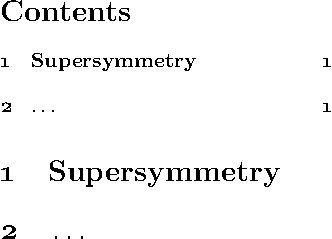
\includegraphics[width = .35\textwidth]{images/Oldtoc.pdf} \kern4\ccwd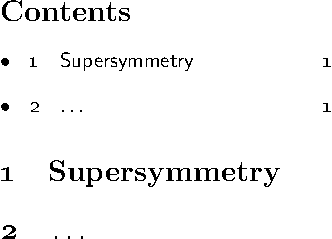
\includegraphics[width = .35\textwidth]{images/Newtoc.pdf}
				\end{center}
			\end{block}
		\item<+-> \pkg{etoolbox} 宏包.偷偷修改(补丁)默认的定义(?).
	\end{itemize}
\end{frame}

\begin{frame}[fragile]{新闻:取所好者}
	\begin{itemize}
		\item<+-> |texdoc ltnews|
		\item<+-> LaTeX Companion 3 发售了;
		\item<+-> \LaTeX{} Hooks.拦截宏展开;
		\item<+-> 整数和浮点数基本计算默认调用: |\inteval|、|\fpeval|;
		\item<+-> 命令和环境复制器.|\NewEnvironmentCopy|(暂未更新)、|\NewCommandCopy|.
	\end{itemize}
\end{frame}

\begin{frame}[fragile]{彩色盒子}
	\begin{tcolorbox}[enhanced,title={\heiti 你想要},frame style image=blueshade.png,colback = 碧蓝!4]
		这样的盒子吗?
		\tcblower
		使用 \pkg{tcolorbox} 宏包!文档:|texdoc tcolorbox|;或者用 |texdoc tcolorbox-example| 查看例子.
	\end{tcolorbox}
\end{frame}

\begin{frame}{文字类排版:字体}
	\begin{itemize}
		\item<+-> 对中文使用者来说,一般使用 \pkg{fontspec} 宏包.
			\begin{itemize}
				\item \CTeX{} 宏集的策略大致是,将 Unicode 字符分成不同的类,每一类单独处理.比如:中文和英文用的就是不一样的字体.
				\item \JPtext{日本語}.当作者意欲在中文内插入日文时,自然应该使用日文字体:
				      \begin{center}
					      八坂神奈子\kern\ccwd 与\kern\ccwd \JPtext{八坂神奈子}
				      \end{center}
				      而不是使用中文字体,这大抵上是最容易出错的细节.
				\item 繁体中文和韩语类似.大陆字体会做日文、韩文部分不代表可以用其来排日文、韩文.
			\end{itemize}
		\item<+-> 如果作者发给你的是 Word 文档,可以先好好沟通一下格式应当如何处理.
	\end{itemize}
\end{frame}

\begin{frame}{文字类排版:OpenType 特性}
	\begin{itemize}[<+->]
		\item 连字:f{}f $\to $ ff, f{}i $\to $ fi, f{}l $\to $ fl;
		\item 老式数字(\texttt{onum}):0123456789 $\to $ {\addfontfeatures{RawFeature={+onum}}0123456789};
		\item 小写大写字母(\texttt{smcp}):An Academic Fantasy For Minority $\to $ {\addfontfeatures{RawFeature={+smcp}}An Academic Fantasy For Minority};
		\item \texttt{case} 特性:{\addfontfeatures{RawFeature={-case}}(西文括号配中文)} $\to $ (西文括号配中文);
		\item 想要知道自己手上字体的 OpenType 特性?\link{https://fontdrop.info}
	\end{itemize}
\end{frame}

\begin{frame}[fragile]{文字类排版:一些碎碎念}
	\begin{itemize}[<+->]
		\item {\bfseries \CJKfontspec[AutoFakeBold = 3]{NotoSerifCJKsc-Medium.otf} 伪粗体}和{\itshape\CJKfontspec[AutoFakeSlant = .16666]{NotoSerifCJKsc-Medium.otf} 伪斜体}.正文中各种意义上都不推荐.但需说明的是,伪斜体可以用在排版代码中的注释.
		\item 罗马数字.{\fontspec{Noto Serif CJK SC Medium}Ⅰ}--{\fontspec{Noto Serif CJK SC Medium}ⅹ},\texttt{U+2160–217F}. Unicode 标准声称收容罗马数字乃是为了兼容性之举,对大多数目的而言应用恰当的拉丁字母列替代之.
		\item 引号.目前常用的蝌蚪形引号有四种(不分中英):
		      \begin{center}
			      \begin{tblr}{cccc}
				      \texttt{U+201C}                                     & \texttt{U+201D}                               & \texttt{U+2018}                                     & \texttt{U+2019}                               \\
				      \makebox[.5\ccwd][l]{\ccbox}\makebox[.5\ccwd][r]{“} & \makebox[0pt][l]{\ccbox}\makebox[\ccwd][l]{”} & \makebox[.5\ccwd][l]{\ccbox}\makebox[.5\ccwd][r]{‘} & \makebox[0pt][l]{\ccbox}\makebox[\ccwd][l]{’}
			      \end{tblr}
		      \end{center}
		      对 \LaTeX{} 和 \CTeX{} 来说,输入以上四种会调用中文字体的全宽引号.欲得到调用西文字体的引号请输入 |`| 和 |'|.
		\item 破折号.破折号可以说是最难以处理的标点,目前没有完美的解决方案.\link{https://github.com/CTeX-org/ctex-kit/issues/382}
	\end{itemize}
\end{frame}

\begin{frame}[fragile]{喜欢的宏包}
	\begin{multicols}{3}
		\begin{itemize}
			\item 必备

			      \begin{itemize}
				      \item \pkg{amsmath}
				      \item \pkg{graphicx}
				      \item \pkg{hyperref}
			      \end{itemize}
			\item 样式

			      \begin{itemize}
				      \item \pkg{caption}
				      \item \pkg{enumitem}
				      \item \pkg{fancyhdr}
				      \item \pkg{geometry}
			      \end{itemize}
			\item 数学

			      \begin{itemize}
				      \item \pkg{bm}
				      \item \pkg{mathtools}
				      \item \pkg{physics2}
				      \item \pkg{unicode-math}
			      \end{itemize}
			\item 表格

			      \begin{itemize}
				      \item \pkg{array}
				      \item \pkg{booktabs}
				      \item \pkg{longtable}
				      \item \pkg{tabularx}
				      \item \pkg{tabularray}
			      \end{itemize}
			\item 插图、绘图

			      \begin{itemize}
				      \item \pkg{subfig}
				      \item \pkg{tikz}
				      \item \pkg{pgfplots}
			      \end{itemize}
			\item 字体

			      \begin{itemize}
				      \item \pkg{newtx}
				      \item \pkg{newpx}
				      \item \pkg{pifont}
				      \item \pkg{fontspec}
			      \end{itemize}
			\item 杂项功能

			      \begin{itemize}
				      \item \pkg{beamer}
				      \item \pkg{biblatex}
				      \item \pkg{fancyhdr}
				      \item \pkg{listings}
				      \item \pkg{mhchem}
				      \item \pkg{siunitx}
				      \item \pkg{xcolor}
			      \end{itemize}
		\end{itemize}
	\end{multicols}
\end{frame}


\begin{frame}[standout]
    \Huge\ttfamily\textbackslash end\{document\}
\end{frame}
\end{document}